\section{Problem and Measurement Model}
\label{sec:narrative-problem}

At report $k$, inference uses measurements through $t_k=k/30$ to decide
whether a physical intervention occurred. Detection concerns its presence;
classification selects a physical operator; localization selects a bus or
branch. These outputs can become reliable at different times. We record
the estimated physical onset $\widehat\tau$ separately from the alarm and
diagnosis emission times.

Figure~\ref{fig:reference-event-types} introduces the broader measurement
phenomena using the known RAW0001 reference record. Faults, line changes,
generation changes and load changes alter the physical network; missing or
corrupted reports alter observation integrity. The present causal test
addresses load changes and line openings with restoration. The other panels
provide context, not additional validated event classes.

\begin{figure*}[t]\centering
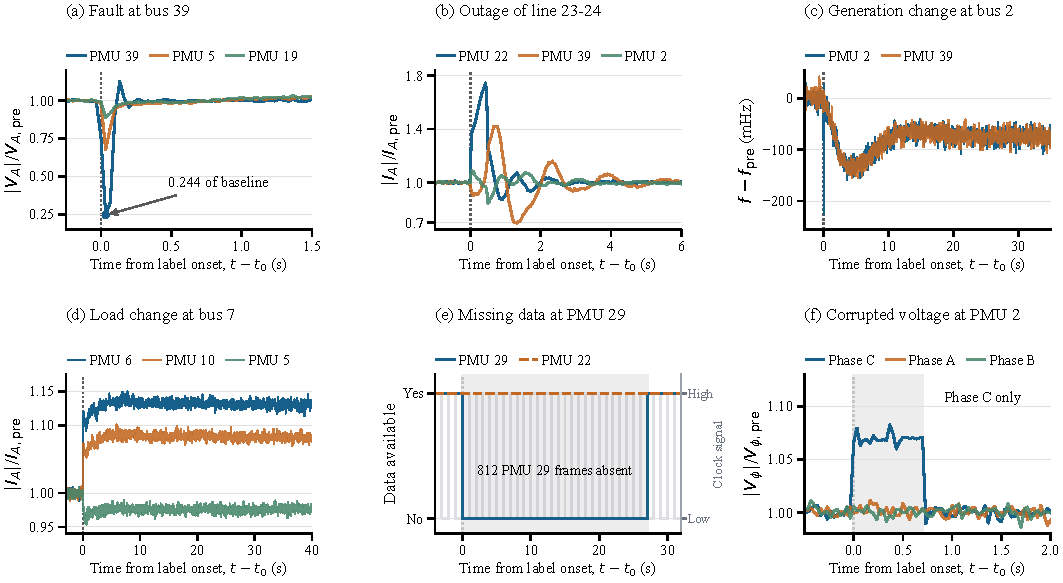
\includegraphics[width=.98\textwidth]{figures/generated/event_signatures.pdf}
\caption{Representative signatures from the archived RAW0001 reference simulation: fault, line outage, generation change, load change, missing PMU data and corrupted voltage. Alignment uses retrospective label onset for illustration; inference receives no such alignment. The gray clock in (e) is an illustrative reference, not another measured channel. Only load and line mechanisms enter the causal evaluation below. RAW0001 is known retrospective evidence, not independent field validation.}
\label{fig:reference-event-types}\end{figure*}

The network has 39 buses, but the prescribed PMU set is
\begin{equation}
 \mathcal P=\{2,5,6,10,19,22,29,39\}.
 \label{eq:narrative-pmus}
\end{equation}
Voltage is measured at each PMU bus. Current is measured at a specified branch terminal, which can differ from that bus. The causal implementation uses 47 coordinates: eight voltage magnitudes, eight voltage angles, eight current magnitudes, seven current angles, eight absolute frequencies and eight ROCOFs, at 30 reports/s. BUS39 current angle is excluded because its interpretation remains partially validated. The BUS5 current terminal retains the provisional historical 5--6 assignment. These are declared measurement assumptions, not identities inferred from classification accuracy.

The exported magnitudes are in V and A, angles in degrees, frequency in Hz
and ROCOF in Hz/s. Internal centered coordinates do not replace the
absolute frequency contract. These are reporting-rate phasor measurements;
waveform harmonics or THD are not measured by these channels.

% PROTECTED FIGURE: retain this single-column IEEE-39 diagram. See AGENTS.md.
\begin{figure}[t]\centering
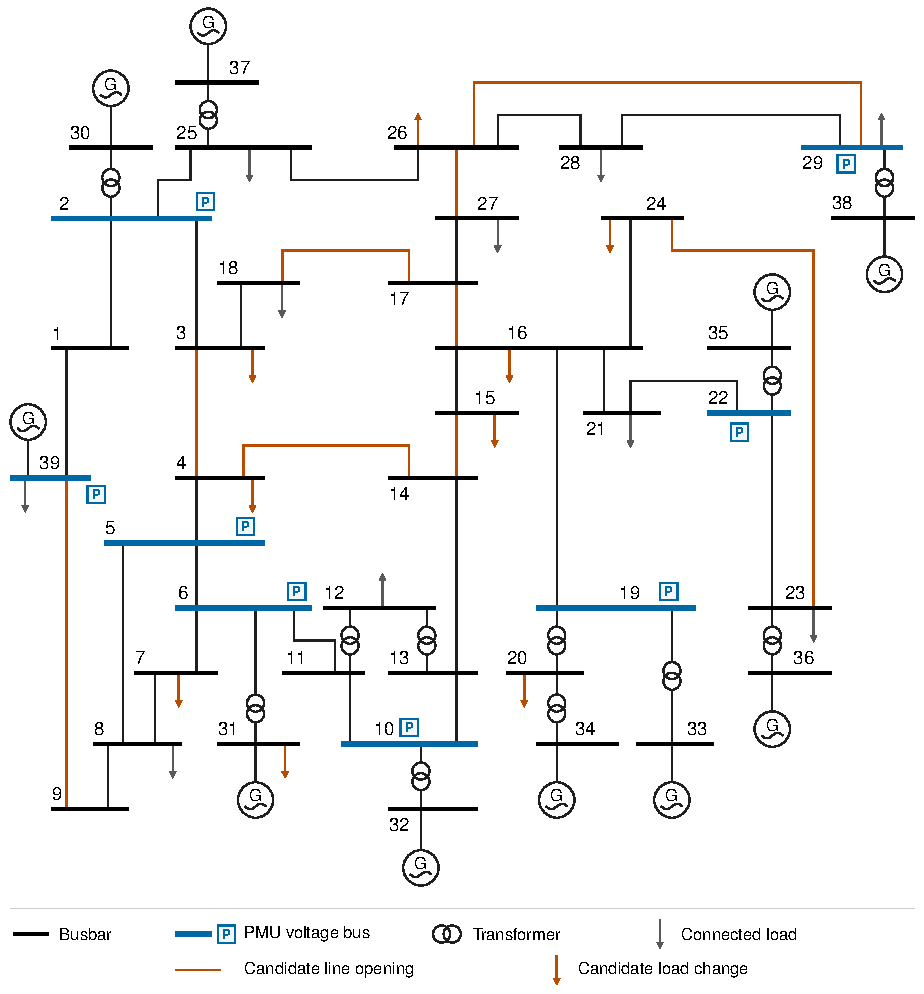
\includegraphics[width=\columnwidth]{figures/generated/narrative_topology.pdf}
\caption{IEEE 39-bus single-line diagram: 46 branches, 12 transformers and 10 generators. Blue bars and P marks locate the eight voltage PMUs. Orange branches and load arrows identify the nine line and nine load candidates; gray arrows denote other loads. Current terminals follow the separate measurement contract. All routes are orthogonal.}
\label{fig:narrative-topology}\end{figure}

The physical model is
\begin{align}
 \dot x&=f_q(x,z,u;\theta),&0&=g_q(x,z,u;\theta),\label{eq:narrative-dae}\\
 y_k&=\mathcal M_q(x_k,z_k;\theta_M)+b+\varepsilon_k.\label{eq:narrative-measurement}
\end{align}
Here $x$ contains machine and control dynamics, $z$ the algebraic network variables, $q$ the topology/intervention mode, and $\theta_M$ the measurement convention. The measurement map includes gains, phase references, orientation and the causal frequency/ROCOF estimator. A machine's rotor speed is not substituted for bus frequency.

An intervention history is $h=(e,c,\tau,a,\kappa)$: family, source, onset,
severity and restoration time, with $\kappa=\infty$ for a sustained event.
Its duration is $\kappa-\tau$ when restoration occurs. A load changes its
local P/Q setpoints; a line opening switches its branch primitive. For the
supported impulse-free switches,
\begin{equation}
 x(\tau^+)=x(\tau^-),\qquad g_{q^+}(x(\tau^-),z(\tau^+),u;\theta)=0.
 \label{eq:narrative-switch}
\end{equation}
The algebraic voltage/current response may jump even though dynamic states remain continuous. Physical restoration reverses the intervention operator. It does not return the machines to their pre-event state, so electrical recovery can continue after OFF.

\begin{table}[t]\centering\small
\caption{Scope of the executed causal component. The source is an intervention asset; it is not necessarily a measured PMU bus.}\label{tab:narrative-scope}
\begin{tabularx}{\columnwidth}{@{}lXX@{}}\toprule
Case & Physical operator & Executed claim\\\midrule
Normal & No intervention & Monitor after startup\\
Load & Local P/Q factor; optional restoration & Nine candidate buses\\
Line & Branch open; optional reclose & Nine candidate branches\\
Fault/generation & Different shunt/input/trip operators & Outside this causal test\\
Missing/bad data & Measurement-integrity mechanism & Outside C01\\
Unknown & Unresolved diagnosis & Not a new physical family\\\bottomrule
\end{tabularx}\end{table}

The generator stores event schedules and true states separately from the PMU stream. Inference receives the nominal network, permitted calibration and reports through the current time. It receives no source, switch time, true R/X realization or solver state. Initial operating context and noise scale are estimated from 300 startup reports; monitoring begins after the inherited 12-s warmup. The startup contract assumes no intervention in that prefix.
